\documentclass[a4paper,12pt]{article}
%\usepackage{fullpage}
%\usepackage{pdfpages}

\usepackage{geometry}
 \geometry{
 a4paper,
 total={170mm,257mm},
 left=20mm,
 top=20mm,
 }

\usepackage{color}
\usepackage{amsmath,graphicx,makeidx}
\usepackage{lscape}
\usepackage{fancyhdr}
\addtolength{\headheight}{1.5cm} % make more space for the header
\pagestyle{fancyplain} % use fancy for all pages except chapter start
\lhead{
\includegraphics[height=1.7cm]{FOSSEE-logo}} % left logo
\rhead{
\includegraphics[height=3.5cm]{DWSIM-flowsheeting-project-logo}} % right logo
\renewcommand{\headrulewidth}{0pt} % remove rule below header

\title{Natural Gas Processing Unit}
\author{Daniel Wagner \\ DWSIM Developer}
\date{}

\begin{document}

\maketitle

\noindent \textbf{Background \& Description:}
\newline One of the important processes in chemical engineering is the processing of natural gas. Moreover, improved production methods due to an increased supply and decreased cost of natural gas, have made the process much more significant. Though the composition of natural gas varies from source to source, it is mostly constituted by methane (70\%) with a small amount of ethane, propane, n-butane, isobutane and heavier hydrocarbons. $C_2$ and heavier hydrocarbons are more valuable than methane and hence it is very important to recover them. $C_2$ and heavier hydrocarbons are called as ‘Natural Gas Liquid’. Recovery is accomplished in a series of three distillation columns. 

Recovery of hydrocarbons from the natural gas feed is achieved by using a series of distillation columns. First, industrial methane is separated in a high pressure cryogenic distillation column using expansion. The column is called demethanizer and is designed in a way to keep a low concentration of methane in its bottom product. The column is operated at 10 kgf/cm$^2$.
Deethanizer is the second column, used in the process to recover industrial ethane. The column operates at 7 kgf/cm$^2$. Refrigeration is used in the condenser and the column is designed in such a way that the distillate only has a specified concentration of propane impurity. 
Debutanizer is the third column, used in the process to recover $C_3$ and $C_4$ which are in higher concentration as the distillate known as LPG. The column is operated at 5 kgf/cm$^2$. The bottom stream contains $C_5$ in high concentration along with traces of other hydrocarbons known as Natural Gasoline.

\vspace{25mm}
\centerline{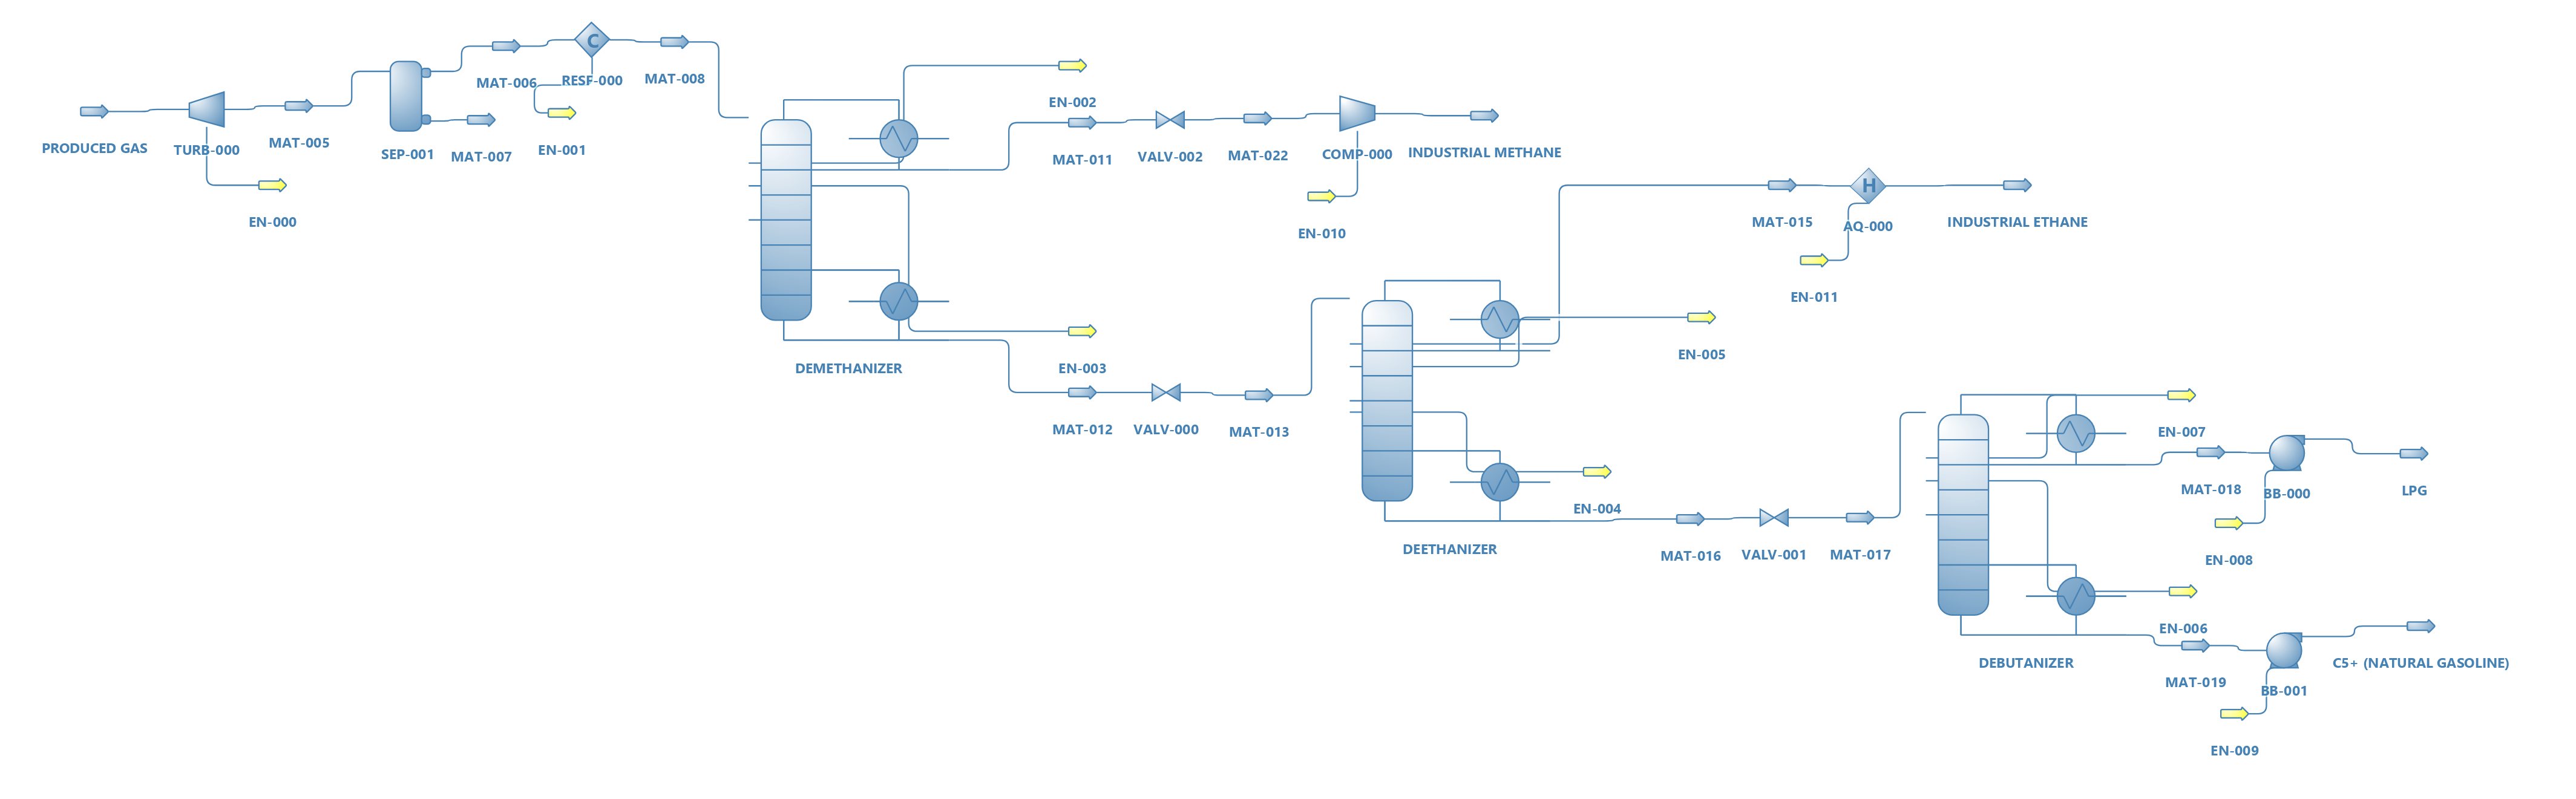
\includegraphics[width=1.15\linewidth]{Nat-Gas.png}}

\newpage
\noindent \textbf{Results:}
\begin{table}[ht]
\centering
\resizebox{\textwidth}{!}{%
\begin{tabular}{|l|l|l|l|l|l|l|}
\hline
\bf Object                                     & PRODUCED & LPG      & INDUSTRIAL         & INDUSTRIAL        & C5+ (NATURAL           &           \\
                                     		   & GAS      &          & METHANE            & ETHANE            & GASOLINE)              &           \\ \hline
Temperature                                & 32           & 18.81856 & -140.492           & 42.04431          & 88.22132               & C         \\ \hline
Pressure                                   & 40           & 19.98    & 8.35868            & 7                 & 10                     & kgf/cm$^2$   \\ \hline
Mass Flow                                  & 41363.93     & 7125.386 & 23480.96           & 6088.564          & 380.4179               & kg/h      \\ \hline
Molar Flow                                 & 1001474      & 76998.98 & 773544.4           & 105000            & 3000                   & m$^3$/d @ SC \\ \hline
Molar Fraction (Mixture)  /  Methane       & 0.698        & 0        & 0.89845            & 0.01627           & 0                      &           \\ \hline
Molar Fraction (Mixture)  /  Ethane        & 0.08725      & 0.01628  & 0                  & 0.79656           & 0                      &           \\ \hline
Molar Fraction (Mixture)  /  Propane       & 0.05235      & 0.42343  & 0                  & 0.13399           & 0.00001                &           \\ \hline
Molar Fraction (Mixture)  /  n-Butane      & 0.02         & 0.1562   & 0                  & 0.00803           & 0.00245                &           \\ \hline
Molar Fraction (Mixture)  /  i-Butane      & 0.0401       & 0.34088  & 0                  & 0.02478           & 0.00133                &           \\ \hline
Molar Fraction (Mixture)  /  i-Pentane     & 0.0087       & 0.04255  & 0                  & 0.00078           & 0.09914                &           \\ \hline
Molar Fraction (Mixture)  /  n-Pentane     & 0.0131       & 0.02066  & 0                  & 0.00075           & 0.89708                &           \\ \hline
Molar Fraction (Mixture)  /  Nitrogen      & 0.0785       & 0        & 0.10155            & 0                 & 0                      &           \\ \hline
Molar Fraction (Mixture)  /  CarbonDiOxide & 0.002        & 0        & 0                  & 0.01883           & 0                      &           \\ \hline
\end{tabular}%
}
\caption{Streamwise Results for Natural Gas Processing Unit}
\end{table}

\end{document}


